% do not change these two lines (this is a hard requirement
% there is one exception: you might replace oneside by twoside in case you deliver 
% the printed version in the accordant format
\documentclass[11pt,titlepage,oneside,openany]{book}
\usepackage{times}


\usepackage{graphicx}
\usepackage{latexsym}
\usepackage{amsmath}
\usepackage{amssymb}

\usepackage{ntheorem}
\usepackage{listings}           

% \usepackage{paralist}
\usepackage{tabularx}

% this packaes are useful for nice algorithms
\usepackage{algorithm}
\usepackage{algorithmic}

%this package adds " " after commands, allows us a nicer
%formatting of texts
\usepackage{xspace}
\usepackage[colorlinks = false, pdfborder={0 0 0}]{hyperref}
\usepackage[authoryear]{natbib}

% well, when your work is concerned with definitions, proposition and so on, we suggest this
% feel free to add Corrolary, Theorem or whatever you need
\newtheorem{definition}{Definition}
\newtheorem{proposition}{Proposition}


% its always useful to have some shortcuts (some are specific for algorithms
% if you do not like your formating you can change it here (instead of scanning through the whole text)
\renewcommand{\algorithmiccomment}[1]{\ensuremath{\rhd} \textit{#1}}
\def\MYCALL#1#2{{\small\textsc{#1}}(\textup{#2})}
\def\MYSET#1{\scshape{#1}}
\def\MYAND{\textbf{ and }}
\def\MYOR{\textbf{ or }}
\def\MYNOT{\textbf{ not }}
\def\MYTHROW{\textbf{ throw }}
\def\MYBREAK{\textbf{break }}
\def\MYEXCEPT#1{\scshape{#1}}
\def\MYTO{\textbf{ to }}
\def\MYNIL{\textsc{Nil}}
\def\MYUNKNOWN{ unknown }
% simple stuff (not all of this is used in this examples thesis
\def\INT{{\mathcal I}} % interpretation
\def\ONT{{\mathcal O}} % ontology
\def\SEM{{\mathcal S}} % alignment semantic
\def\ALI{{\mathcal A}} % alignment
\def\USE{{\mathcal U}} % set of unsatisfiable entities
\def\CON{{\mathcal C}} % conflict set
\def\DIA{\Delta} % diagnosis
% mups and mips
\def\MUP{{\mathcal M}} % ontology
\def\MIP{{\mathcal M}} % ontology
% distributed and local entities
\newcommand{\cc}[2]{\mathit{#1}\hspace{-1pt} \# \hspace{-1pt} \mathit{#2}}
\newcommand{\cx}[1]{\mathit{#1}}
% complex stuff
\def\MER#1#2#3#4{#1 \cup_{#3}^{#2} #4} % merged ontology
\def\MUPALL#1#2#3#4#5{\textit{MUPS}_{#1}\left(#2, #3, #4, #5\right)} % the set of all mups for some concept
\def\MIPALL#1#2{\textit{MIPS}_{#1}\left(#2\right)} % the set of all mips


\begin{document}

\lstset{language=HTML} 
\pagenumbering{roman}
% lets go for the title page, something like this should be okay
\begin{titlepage}
	\vspace*{2cm}
  \begin{center}
   {\Large Extraction of Goals from Premier League Match Reports using Natural Language Processing Techniques\\}
   \vspace{2cm} 
   {Student  Project\\}
   \vspace{2cm}
   {presented by\\
    Jochen H\"{u}l\ss \xspace  \&  Matthias Rabus \\
    Matriculation Number 1376749 \& 1207834 \\
   }
   \vspace{1cm} 
   {submitted to the\\
    Chair of Information Systems V\\
    Prof.\ Dr.\ Christian\ Bizer\\
    University Mannheim\\} \vspace{2cm}
   {Mai 2013}
  \end{center}
\end{titlepage} 

% no lets make some add some table of contents
\tableofcontents
\newpage

%\listofalgorithms

\listoffigures

%\listoftables

% evntuelly you might add something like this
% \listtheorems{definition}
% \listtheorems{proposition}
\newpage


% okay, start new numbering ... here is where it really starts
\pagenumbering{arabic}

\chapter{Project Summary}
\section{Application Domain and Goals}
\label{sec:goals}

In recent years our society underwent a remarkable change in terms of the ubiquitous availability of electronically-written text. The reader might think of the rise of e-ink interfaces and the subsequent shift from print media to electronic books, papers, magazines and so forth. Apart from editorial content, a massive development of informal information sources has been taken place.\\ 
On the one hand, the blogosphere puts the right of speech on an entirely new level. On the other hand, numerous possibilities have been emerging to customers reviewing, recommending and, thus, influencing the perception of products and services in a written way. Automatically retrieving structured information from these various sources of written text is yet a challenging task \citep[p.1]{Cellier2010}. However, robust models in this domain can even help gaining a more transparent overview in emergency situations such as disaster relief by analyzing Twitter feeds.\\

Due these plentiful reasons, the domains of text mining and Information Extraction (IE) have drawn their attention to us. Both domains tied together enable the automatic identification of selected types of entities, relations, or events in free text \citep[p.545]{Grishman2005}. Our research interest and also project goal is two-fold. Firstly, we want to find and apply patterns extracting a particular event from an unknown textual source. Secondly, the robustness of the patterns found should be assessed by classifying an unlabeled source. According to \citeauthor*{Weiss2005} \citeyearpar{Weiss2005} the first task can be referred to as Information Retrieval because we provide "clues" that determine the matching documents. They also argue that the second task is considered as a Document Classification one.\\

More specifically, we want to exemplify written football match reports from England's Premier League to investigate whether the event of a goal can be mined for automatically. With the help of manually-found seeds, our hypothesis is that a model classifying a document according to the occurrence of a goal with an accuracy of at least 75\% is achievable based on automatically-labeled training data. Moreover, the model found should also work on a sample unknown and unlabeled match report.\\

The research report is comprised of a description of the obtained data set [\ref{sec:structure}], our various preprocessing steps [\ref{sec:preproc}], the applied web data mining methods [\ref{sec:webmining}] as well as an evaluation of our results [\ref{sec:eval}].


\section{Structure and size of the data set}
\label{sec:structure}

Since many NLP tools work best with English language, we would like to increase our chance of success by using football reports of the English Premier League. The BBC sports department offers match reports for every game of the currently ongoing season 2012/2013. The amount of reports is sufficient for the purpose of this project. A Premier League season consists of 38 match days with 10 games each. BBC provides one report per game. The BBC sports department is a good data source because the reports are neutrally written and have no preference for any team. Furthermore, the used language has got a higher level and should be, compared to spoken word, easier to analyze. \\

The first step is gathering the data from the BBC homepage. Crawling the data will be described more detailed in the following section~\ref{sec:preproc} about preprocessing. These data was the input for the following classification process. Thus we wanted to classify each sentence whether it contained a goal or not, we had to generate a sentence-wise input first.  The result of our crawling process was one HTML file per report. Like every HTML file, our results had a nested tree structure including some JavaScript and CSS, as well. A problem occurred was that the text fragments themselves contained HTML tags, for example references to other reports. For extracting the plain text from the rest of the HTML documents, we employed XPATH. Then we had to divide each football text into the sentences themselves. This on itself is a challenging task, because a punctuation mark could be a non-sufficient separator, for example if we consider the name of the stadium "St. James Park". The extracted sentences will be a sufficient input for the further research.\\

As we started the research several match days before the end of the Premier League season, our data set comprises a total of 342 football match reports.

\section{Preprocessing}
\label{sec:preproc}
\subsection{Defining Manual Patterns}
As outlined in the previous section, the project started with gathering the data. We used RapidMiner to crawl the data for us. RapidMiner is an open source data mining tool developed by rapid-i.com. RapidMiner allows the user to define a so-called process, which is a combination of certain operators. The operators are connected by defined in- and outputs and can be parameterized to perform specific actions. \\
RapidMiner provides an operator to crawl the World Wide Web. BBC's Premier League result page is structured as follows: It has a main site from which every game report is liked. The reports are grouped by the day of the match. The first task of the crawler is to find the links to the game reports within the results page and then download each linked page into a seperate HTML file. Then the text has to be extracted from the HTML files. Therefor we use RapidMiner as well. The RapidMiner process takes all HTML files and extracts the plain text. This is achieved with the Cut Document-operator and an XPath-query. The extracted text is then written to one file for all reports because the Write as Text-operator can not write into multiple files. \\ 

Afterwards we had to do two steps in parallel. First we had to seperate the text file that contained the whole text from all reports and second we had to manually generate patterns that described goals.
For both tasks some helpful methods were implemented in Java. To use the text for our classifier, it had to be splitted into sentences and each sentence had to be written into an seperate file. Accomplishing this task we used a build-in Java class: BreakIterator. The class provides a method that can cut a given text into sentences given a specific language, English in this case. The previous preprocessing step created some additional lines of text, for example for every new processed file, that also have been removed within this step. As mentioned before, the results of the text splitting were saved and written into seperate text files for further use, but also processed to find some sentences containing goals and some counter examples. \\

If we want to train a classifier to distinguish the sentences for us, we will first have to create examples. Thus, there are rarely two similar sentences describing a goal, you can find certain patterns if you analyze sentences using Natural Language Processing (NLP) tools. "Natural Language Processing is a theoretically motivated range of computational techniques for analyzing and representing naturally occurring texts at one or more levels of linguistic analysis for the purpose of achieving human-like language processing for a range of tasks or applications." \citep[p.1]{Liddy2001} To construct sufficient patterns, we needed two elements of Natural Language Processing: Named Entity recognition (NER) and Part-of-Speech tagging (POS). POS assigns to each word its part of speech tag. It determines if it is a verb, noun, adjective, etc \citep[p.219]{Voutilainen2005}. Whereas, NER determines if a word is an entity, for example a name, a place or a city.  
The \hyperlink{http://nlp.stanford.edu/software/CRF-NER.shtml}{Stanford NLP Group} provides a useful Java library with many build-in language processing tools, including NER and POS tagging. Using this library, we were able to print out a sentence including named entities and part-of-speech tags. We did this for four match reports to manually detect patterns. In total, we were able to extract 14 generic patterns indicating the scoring of a goal. One of the inferred patterns is displayed in Figure~\ref{fig.manualpattern}. \\
\begin{figure} [h!]
\centering
\begin{lstlisting}[frame=single]
[PERSON POS * NN IN * corner]
\end{lstlisting}
\caption{Manual Pattern for "Rooney's volley from Mata's corner."}
\label{fig.manualpattern}
\end{figure}

\subsection{Possibilities of Automated Pattern Matching}
\label{sec:automatch}
As the next preprocessing step, the manual patterns had to be applied on our entire corpus of football match reports in order to find more positive training data for the subsequent classification in an automated way. For this task a search engine capable of querying for n-grams consisting of POS tags, recognized named entities, free tokens, and an arbitrary number of wildcards is needed. A n-gram is a sequence containing n literals.\\
A comprehensive search engine for n-grams has been developed by \citeauthor*{Sekine2010} \citeyearpar{Sekine2010}. Their published work depicts a search engine capable of querying up to 7-grams with POS tags, named entities, and free tokens. The user interface is conveniently web-based. However, their search engine is not publicly accessible and restricted to Wikipedia articles. Moreover, their solution lacks a support of an arbitrary number of wildcards.\\

A thorough analysis of alternatives, also taking an own implementation into consideration, lead us the way to GATE, the "General Architecture for Text Extraction". \citeauthor*{Cunningham2002} \citeyearpar[p.1]{Cunningham2002} states about their tool that "[t]he GATE architecture has enabled us not only to develop a number of successful applications for various language processing tasks (such as Information Extraction), but also to build and annotate corpora and carry out evaluations on the applications generated." A more detailed look on GATE unveiled its powerful and extensive baseline function set. By default, GATE provides a pipeline of text processing resources for common NLP tasks. For instance, a tokeniser, a sentence splitter, a POS tagger, a named entity gazetteer, and an orthomatcher discovering relations between entities and assigning new annotations to tokens \citep[p.5]{Cunningham2002}. Each processing module can be separately added to a processing pipeline and then applied on language resources such as plain text, html, pdf, etc. employing GATE's GUI.\\ 

Apart from standard components, GATE exposes interfaces to extend its processing resources to user's requirements. One of these is the Java Annotation Patterns Engine (JAPE). JAPE was also introduced by \citeauthor*{Cunningham1999} \citeyearpar{Cunningham1999}. According to them, "[a] JAPE grammar consists of a set of phases, each of which consists of a set of pattern/action rules, and which run sequentially". Sequential pattern mining \citep{Agrawal1995} incorporates the concept that sequences of elements can repeatedly occur in a data set and thus form patterns. This idea is essential for IE and makes JAPE grammar rules a viable solution to automatically label unknown language resources derived from manually-inferred patterns. "Patterns can be specified by describing a specific text string, or annotations previously created by modules such as the tokeniser, [POS tagger], gazetteer, or document format analysis" \citep[p.5]{Cunningham2002}. A sample JAPE grammar rule depicting the manual pattern of Figure~\ref{fig.manualpattern} is shown in Figure~\ref{fig.jape}.\\

\begin{figure} [h!]
\centering
\begin{lstlisting}[frame=single]
Rule: Goal3
(
  ({Person.rule == PersonFinal}|{Token.category == NNP}
   |{Lookup.majorType == country_adj})
  {Token.category == POS}
  ({Token.length > 1})*
  ({Token.category == NN}|{Token.category == NNS})
  {Token.category == IN} 
  ({Token.length > 1})*
  {Token.string =~ corner}
)
:goalSequence -->
  :goalSequence.Goal = {kind=Goal, rule=Goal3}
\end{lstlisting}
\caption{Jape Grammer Rule for "Rooney's volley from Mata's corner."}
\label{fig.jape}
\end{figure}

The final preprocessing step became necessary due to GATE's restricted export capabilities. GATE outputs its annotations only as XML tags. These indicate the starting and end character position of a  positively-labeled sentence within the entire text corpus. I.e., we were bound to parse this XML tree with respect to the goal entity. This purpose served the Java API for XML Processing and some routines to write each positive and a corresponding number of negative sentences into a file. After all, we faced an evenly-distributed set of automatically-labeled sentences.

\section{Actual Web Mining}
\label{sec:webmining}
After generating the input for our model we had to find a good model for our preprocessed data. Therefor we experimented with three different approaches: Na\"{i}ve Bayes, Support Vector Machine (SVM) and k-Nearest Neighbor (k-NN) classifier. \\ 
The detailed results will be discussed in the following section. This section provides an overview of the structure of the processes. Each process starts with importing the data into the process.
This operator includes three sub-operators, which split the text into words (Tokenize), then filter stop words and certain words like season, half and minutes. The last operator is configured manually. The next operator balances the number of inputs because there are more sentences containing no goal, then ones including goals. Following the balancing we used a so-called Validation operator in which the model was learned, applied to the data and the performance of our results were measured. \\
\begin{itemize}
\item Na\"{i}ve Bayes \\
The first approach used a Na\"{i}ve Bayes classifier within the validation. "Bayesian classifiers assign the most likely class to a given example described by its feature vector. Learning such classifiers can be greatly simplified by assuming that features are independent given class[. ...] The success of naive Bayes in the presence of feature dependencies can be explained as follows: optimality in terms of zero-one loss (classification error) is not necessarily related to the quality of the fit to a probability distribution [... .] Rather an optimal classifier is obtained as long as both the actual and estimated distributions agree on the most probable class." \citep[p.1]{Rish2001} 
\item Support Vector Machine (SVM) \\
The process remained the same but we changed the model to be a SVM. "Support vector machines are based on the Structural Risk Minimization principle from computational learning theory. The idea of structural risk minimization is to find a hypothesis h for which we can guarantee the lowest true error. The true error of h is the probability that h will make an error on an unseen and randomly selected test example. [...] SVMs are very universal learners. In their basic form, SVMs learn linear threshold function. [...] One remarkable property of SVMs is that their ability to learn can be independent of the dimensionality of the feature space. SVMs measure the complexity of hypotheses based on the margin with which they separate the data, not the number of features." \citep[p.2]{Joachims1998} 
\item k-Nearest Neighbor (k-NN) \\
The most successful attempt used the k-NN technique. "One of the oldest and simplest methods for pattern classification is the k-nearest neighbors (kNN) rule. The kNN rule classifies each unlabeled example by the majority label of its k-nearest neighbors in the training set. Despite its simplicity, the kNN rule often yields competitive results and in certain domains, when cleverly combined with prior knowledge, it has significantly advanced the state-of-the-art. By the very nature of its decision rule, the performance of kNN classification depends crucially on the way that distances are computed between different examples. When no prior knowledge is available, most implementations of kNN compute simple Euclidean distances (assuming the examples are represented as vector inputs). Unfortunately, Euclidean distances ignore any statistical regularities that might be estimated from a large training set of labeled examples." \citep[p.1]{Weinberger2006} We achieved the best results with a k of 50. 
\end{itemize}
Adding the operator "Weight by Information Gain" and "Select by Weights" improved the results as well. The first operator assigns each element of our word vector a normalized value and the second operator selects elements with a weight that is higher then a determined threshold. In our case we achieved the best results using a threshold of 0.05. These two operators replaced the "Sample" operator and improved the results and the runtime of the process, due the size of the data has been reduced.
After the improvement was done, we wanted to use the trained model on unseen data. Therefor we added a "Process Documents"- and an "Apply Model"- operator after the Validation operator. The disadvantage of this was that the results were the sentences itself and the assigned class, so we had to evaluate the results by hand. 

\section{Results and Evaluation}
\label{sec:eval}

The results shown in this section were calculated on the data set introduced in Section~\ref{sec:structure}. After the preprocessing steps the football match reports were split into 9,211 sentences, each of which is separately store as text file. Out of this corpus, the 14 JAPE grammar rules (see Subsection~\ref{sec:automatch}) were able to match and thus extract 758 sentences containing a goal in an unsupervised manner. Given an even number of negative and positive seeds for classification, the following performance measurements base on a total of 1,516 input sentences. The negative seeds were taken randomly from the entire corpus excluding those sentences marked as positive.\\
At first, we attempted to perform the validation of classification models with the complete sentences as attributes. Thus, the classifiers employed 1,498 attributes. However, it turned out to be not a viable solution as none of the classifiers were able to predict a single positive sentence correctly. From these findings we derive that entire sentences are not similar enough to one another to serve as attributes for classification. Hence, the measurements in Subsections~\ref{sec:nb} to~\ref{sec:knn} were conducted with an additional sentence tokeniser and stop-word filter returning now 3,624 word-level attributes for classification.

\subsection{First Iteration: Na\"{i}ve Bayes}
\label{sec:nb}

The measurements of the first iteration employing a Na\"{i}ve Bayes classifier are exposed to the reader in Figure~\ref{fig.nb}. Peculiarly-high is the overall number of positive prediction. Naturally, this yields in a good positive class recall but takes a loss in the negative class recall. Also the positive class precision is not as strong as expected taking into account that the patterns for positive seeds are automatically-labeled though explicitly and precisely defined. The Na\"{i}ve Bayes classifier results in an accuracy of 64.58\%.

\begin{figure} [h!]
\centering
\begin{tabular}{ | l | l | l | l | }
\hline
	 & true neg & true pos & class precision \\ \hline
	pred. neg & 411 & 190 & 68.39\% \\ \hline
	pred. pos & 347 & 568 & 62.08\% \\ \hline
	class recall & 54.22\% & 74.93\% &  \\ \hline
\end{tabular}
\caption{Performance of Na\"{i}ve Bayes classifier}
\label{fig.nb}
\end{figure}


\subsection{Second Iteration: SVM}
\label{sec:svm}

The performance of SVM's classification validation is shown in Figure~\ref{fig.svm}. This result chart has considerably different characteristics from the previous one. As initially expected, the positive class precision is very strong. But by taking into account that the occurrence of positively-predicted sentences is by far fewer than in the Na\"{i}ve Bayesian case, it is obvious that the positive class recall suffers from the good class precision. Thus, the overall accuracy of 70.59\% is higher than in the first iteration, however, is not yet meeting the demand of our hypothesis.

\begin{figure} [h!]
\centering
\begin{tabular}{ | l | l | l | l | }
\hline
	 & true neg & true pos & class precision \\ \hline
	pred. neg & 654 & 342 & 65.66\% \\ \hline
	pred. pos & 104 & 416 & 80.00\% \\ \hline
	class recall & 86.28\% & 54.88\% &  \\ \hline
\end{tabular}
\caption{Performance of Support Vector Machine classifier}
\label{fig.svm}
\end{figure}


\subsection{Third Iteration: Nearest-Neighbor}
\label{sec:knn}

Figure~\ref{fig.knn} depicts the performance sheet of the 50-Nearest-Neighbor method. Strikingly-high is the class recall of positive sentences. As in the first iteration, the 50-NN method buys this figure with trading off its class precision which, in turn, is comparatively low. This high number of positive predictions can be explained through the vast amount of attributes. Those are equally-important for Nearest-Neighbor's distance measurement and, thus, even player names and words such as "bench", "inspiration", or "tense" indicate for the algorithm goals because a positive seed contained them at least once. Nevertheless, the basic application of 50-NN is the first model that holds the hypothesis of an accuracy of at least 75.00\%.

\begin{figure} [h!]
\centering
\begin{tabular}{ | l | l | l | l | }
\hline
	 & true neg & true pos & class precision \\ \hline
	pred. neg & 469 & 90 & 83.90\% \\ \hline
	pred. pos & 289 & 668 & 69.80\% \\ \hline
	class recall & 61.87\% & 88.13\% &  \\ \hline
\end{tabular}
\caption{Performance of Nearest-Neighbor method}
\label{fig.knn}
\end{figure}

\subsection{Fourth Iteration: Weighted Nearest Neighbor}
\label{sec:wknn}
As argued above, the high number of attributes led to a too big positively-classified sentence set. This is because we introduced the Rapidminer operators "Weight by Information Gain" and "Select by Weight" (see Section~\ref{sec:webmining}). We determined that a selection of words with a weight greater than 0.05 yields the best performance. Whereby the top-5 word indicating a goal are "scored", "net", "twice", "corner", and "volley". This restriction only supplies a relatively small number of 235 attributes to the classifier but yet resulting in our best classification model validation shown in Figure~\ref{fig.wknn}. The table unveils a more homogeneously-spread result of precision and recall figures where all are fluctuating around 80\%. This totals in our highest model accuracy of 80.88\%.

\begin{figure} [h!]
\centering
\begin{tabular}{ | l | l | l | l | }
\hline
	 & true neg & true pos & class precision \\ \hline
	pred. neg & 594 & 126 & 82.50\% \\ \hline
	pred. pos & 164 & 632 & 79.40\% \\ \hline
	class recall & 78.36\% & 83.38\% &  \\ \hline
\end{tabular}
\caption{Performance of Weighted Nearest-Neighbor method}
\label{fig.wknn}
\end{figure}

\subsection{Application on sample Match Report}

The findings of the performance measurement in the previous subsections were for training and model validation purposes. To achieve the project goal, the models found are applied on an randomly-chosen, unknown, and unlabeled text, namely the match report of Chelsea vs. Sunderland on April, 7th 2013. We manually counted 24 sentences in the report where eight ones indicate a goal even though the game was only a 2:1 victory for Chelsea. Figure~\ref{fig.appliedmodel} draws the resulting measures for all applied classifiers. As found in the validation steps, the Nearest-Neighbor methods yield again the highest accuracies.


\begin{figure} [h!]
\centering
\begin{tabular}{ | l | l | l | l | l | l | l | }
\hline
	Classifier & \multicolumn{2}{|c|}{Positive} &  \multicolumn{2}{|c|}{Negative} & Accuracy \\ \hline
	& Precision & Recall & Precision & Recall & \  \\ \hline
	Na\"{i}ve Bayes & 0.33 & 0.75 & 0.67 & 0.25 & 50.0\% \\ \hline
	SVM & 0.33 & 0.75 & 0.67 & 0.25 & 50.0\% \\ \hline
	50-NN Basic & 0.64 & 0.92 & 0.88 & 0.75 & 81.3\% \\ \hline
	50-NN Weighted  & 0.71 & 0.63 & 0.82 & 0.88 & 75.0\% \\ \hline
\end{tabular}
\caption{Application of different investigated classification models on a sample report with 24 sentences (8 positive, 12 negative)}
\label{fig.appliedmodel}
\end{figure}

Figure~\ref{fig.plot} depicts a plot of this practical case. The best possible score is in the upper-right corner with a precision of 1 and also a recall of 1. Each classifier has got two data points - a positive and negative one. The best overall plot is scored by 50-NN Weighted negative. However, the best combined plot and, thus, the best accuracy for this specific match report scores the 50-NN Basic model. Yet this proves that our hypothesis holds also on unknown and unlabeled data.

\begin{figure} [h!]
\centering
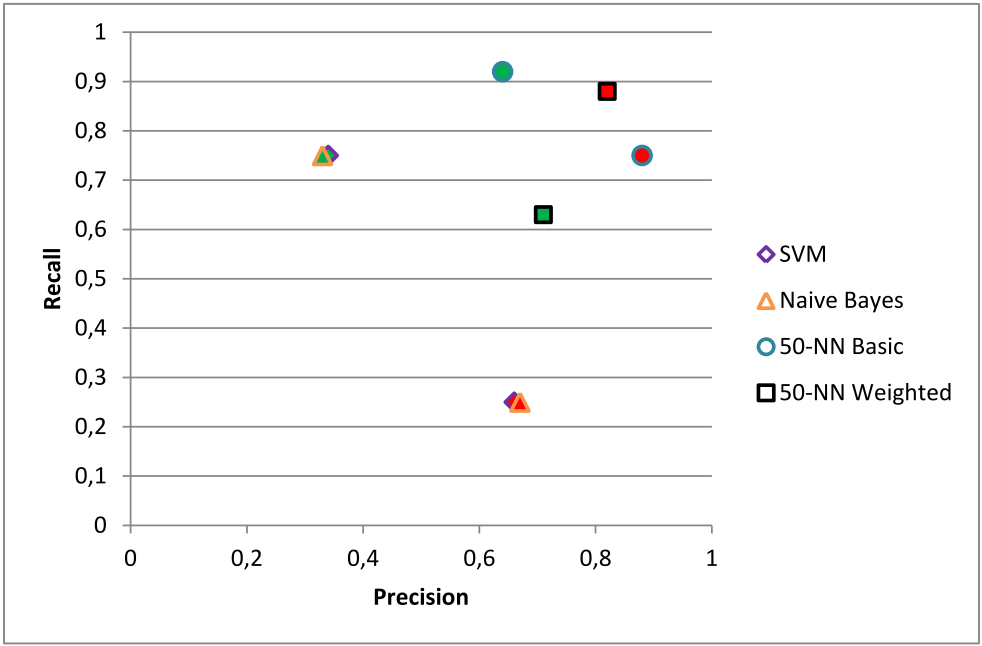
\includegraphics[width=0.7\textwidth]{precRecall.PNG}
\caption{Plot of classification models applied on a sample report (green = positive, red = negative)}
\label{fig.plot}
\end{figure}

\section{Conclusion}
The project paper outlined a way to detect goals in sentences of football match reports. It was possible to train different classifiers to achieve this goal. Based on the given data the kNN method provided the highest success rates. An interesting additional feature is the semi-automated generation of example sentences using GATE and Jape Grammar Rules. They provided the opportunity to generate many examples from some manually created rules.\\
We experimented with three different classifiers - Na\"{i}ve Bayes, Support Vector Machine and k-Nearest Neighbor and different parameter settings. In the end we gained a precision of 76.5\% and a recall of 75.5\% for our kNN process with $k = 50$ using the  operators "Weight by Information gain" and "Select by Weights".\\
Possible challenges for further research could be the determination if a goal is described in multiple sentences or multiple times within a report to conclude the exact result from a given report. Furthermore, you could think about adopting the discussed techniques to other languages, for example German or Spanish. 

\bibliographystyle{apalike}
\bibliography{bibliography}
\end{document}
